% !TeX root = Main.tex

\chapter{Postup řešení úloh v~aplikaci Agros2D}  \label{kap:tutorial}
Analýza fyzikálního pole ve všech programech, zabývajících se touto problematikou, bývá zpravidla rozdělena do třech základních etap. Toto obecné rozdělení je aplikované i~v~programu Agros2D.
\begin{itemize}
\item {\bf PreProcessing} - Prvním krokem je vytvoření modelu a definování jeho geometrických rozměrů. Dále je potřeba zvolit materiálové vlastnosti, nastavit úroveň diskretizace a typ analýzy.
\item {\bf Solution} - V~další části probíhá vlastní řešení požadovaným řešičem.
\item {\bf PostProcessing} - Nakonec se provádí vyhodnocení řešeného problému.
\end{itemize}
Následující postup podrobněji rozepisuje kroky, které vedou k~řešení konkrétních fyzikálních problémů pomocí aplikace Agros2D.
\begin{enumerate}
\item {\bf Vytvoření a nastavení nového problému} - Pomocí dialogu \uv{nastavení problému} (na obrázku \ref{obr:sim_problem_properties}), který se zobrazí po vytvoření nové úlohy, je možné zvolit druh řešeného fyzikálního pole, typu problému a druhu analýzy. Dále lze aktivovat $h$, $p$ nebo $hp$ adaptivitu, nastavit parametry diskretizační sítě a frekvenci.
\begin{figure}[!h]
	\centering
	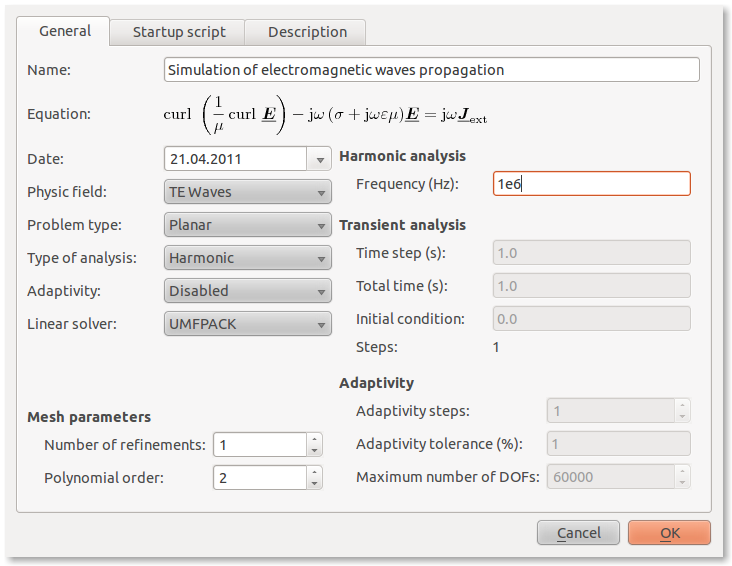
\includegraphics[width=9cm]{sim_problem_properties.png}
	\caption{Dialog \uv{nastavení problému} programu Agros2D.}
	\label{obr:sim_problem_properties}
\end{figure}
\item {\bf Nakreslení struktury} - Geometrii úlohy lze nastavit vložením uzlů a zakreslením hranic mezi nimi. Materiálové konstanty je možné specifikovat značkami oblastí.
\begin{itemize}
\item {\bf Nový uzel} - Po výběru nástroje \uv{práce s uzly} je možné vložit uzel přidržením Ctrl a levým kliknutím myši (případně pomocí dialogu vyvolaném stisknutím \mbox{Alt + N}).
\item {\bf Nová hrana} - Nástrojem \uv{práce s hranami} se vytvoří hranice opět držením Ctrl a kliknutím mezi dva již vytvořené uzly (další možnost tvorby hranic představuje dialog vyvolaný kombinací \mbox{Alt + E}).
\item {\bf Nová značka oblastí} - Tu lze zadat nástrojem \uv{práce se značkami oblastí} přidržením Ctrl a kliknutím na požadované místo (\mbox{Alt + L}).
\end{itemize}
\item {\bf Vytvoření okrajových podmínek} - Pro jejich tvorbu a bližší specifikaci slouží dialog \uv{nová okrajová podmínka}. Ten je možné zpřístupnit po pravém kliknutí na pracovní plochu a vybrání daného odkazu, případně je možné se na něj dostat klávesovou zkratkou \mbox{Alt + B}. Po zadání požadovaného označení se vybere v~rozbalovacím menu některá z~definovaných okrajových podmínek.

Příklad pro zadání Dirichletovy okrajové podmínky, ve formátu reálné a imaginární složky na hranici $\Gamma$ pro hodnotu $0 + \mj 0\unit{V/m}$, je na obrázku \ref{obr:sim_BC_electric_field}. Ta se v~oboru vysokofrekvenční techniky označuje jako \uv{perfect electric conductor}.
\begin{figure}[!h]
	\centering
	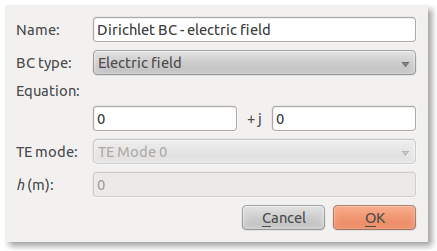
\includegraphics[width=7cm]{sim_BC_electric_field.png}
	\caption{Zadání Dirichletovy podmínky $0 + \mj 0\unit{V/m}$ pro elektrickou složku pole.}
	\label{obr:sim_BC_electric_field}
\end{figure}
\item {\bf Přiřazení vytvořených podmínek na příslušnou hranu} - Toto je možné po dvojkliku na hranu nebo jednoduchým kliknutím lze vybrat více hran a po stisku mezerníku zadat podmínku hromadně.
\item {\bf Vytvoření materiálů} - Nastavení jejich parametrů se děje v~dialogu patrném na obrázku \ref{obr:sim_material}, který znázorňuje zadání materiálu vzduch pro řešení elektromagnetického pole. 
\begin{figure}[!h]
	\centering
	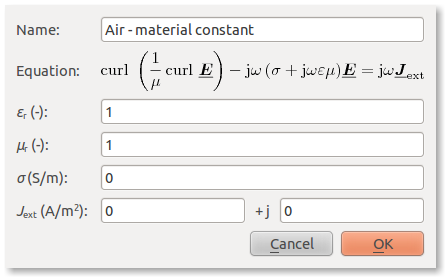
\includegraphics[width=7cm]{sim_material.png}
	\caption{Vytvoření materiálu vzduchu v okně \uv{nový materiál}.}
	\label{obr:sim_material}
\end{figure}
Parametry $\varepsilon_r$ a $\mu_r$ představují relativní hodnoty permitivity a permeability. Pomocí $\sigma$ zadáme vodivost v~daném prostředí. Poslední parametr $J_{\mathrm{ext}}$ představuje vnucený proud do oblasti, která je reprezentovaná danou značkou. Zpřístupnit tento dialog lze opět pravým kliknutím na pracovní plochu a vybráním možnosti \uv{nový materiál}, eventuálně zkratkou \mbox{Alt + M}. 
\item {\bf Přiřazení vytvořených značek k~dané oblasti} - Zadání je možné, obdobně jako u okrajových podmínek, po dvojkliku na značku oblastí. Případně lze využít výběru myší a mezerníku pro hromadné přiřazení.
\item {\bf Diskretizace oblasti} - Globální úroveň se nastavuje při specifikaci problému, lokální nastavení lze provést u~vlastností hrany nebo u~značky oblasti.
\item {\bf Spuštění řešení}
\begin{figure}[!h]
	\centering
	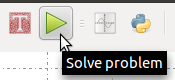
\includegraphics[width=3cm]{sim_spusteni_reseni.png}
\end{figure}
\item {\bf Volba vhodného zobrazení výsledků} - K~tomuto účelu slouží vlastnosti postprocesoru na levé straně pracovní plochy. Je možné například aktivovat nebo skrýt geometrii, diskretizační síť, kontury zobrazení a také odpovídající vektory. Dále lze vybrat zobrazení požadovaných veličin a jejich odpovídajících složek, které se týkají řešení daného fyzikálního pole z~níže patrného rozbalovacího menu.%, které je patrné na obrázku \ref{obr:sim_zobrazeni}.
\begin{figure}[!h]
	\centering
	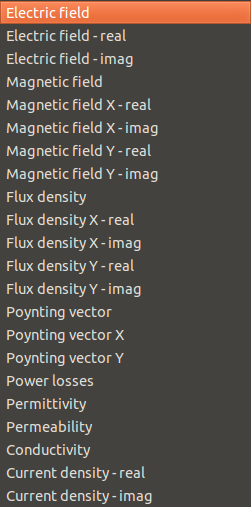
\includegraphics[width=4cm]{sim_zobrazeni.png}
	%\caption{Volba veličiny pro zobrazení.}
	\label{obr:sim_zobrazeni}
\end{figure}
\end{enumerate}


